\chapter{Tools}
\label{cha:Tools}

In order to create the CodeSpeech prototype, multiple different tools were combined together. Because this project was developed as an Eclipse plugin, IDE itself and Plug-In Development Environment (PDE) are used as a development platform. For speech recognition two different toolkits were tested, namely open-source CMUSphinx (in two versions - Pocketsphinx and Sphinx4) and a commercial Google Cloud Speech-to-Text. For analysis of recognized phrases against the grammar file ANTLR parser was utilized. This chapter will introduce and briefly describe each of the aforementioned tools.

\section{Eclipse}

Eclipse is free of charge, open-source Integrated Development Environment. Eclipse is mostly written in Java and primarily used for developing Java applications, although it also allows development in other programming languages such as languages from C family, Python, PHP, JavaScript etc. via plugins. The Eclipse Public License (EPL) is the fundamental license under which Eclipse projects are released. The initial launch was in November of 2001. It can be used at any of the most popular operating systems, such as Linux, Windows, Mac OSX, UNIX. The exemplary view of Eclipse IDE can be seen in Fig. \ref{fig:eclipseIDE}.

It was selected as a development tool and the target platform for three main reasons among others. The first one being, the knowledge of and familiarity with the environment, which the author of this thesis gained during the many years of its use. The second is the fact that Eclipse is easily extendable via plugins (more on that later), therefore it seemed plausible to create an extension for it, especially because it provides a special set of tools that assist in the development of extension (described in the next section). Finally, when doing research about the potential development platforms it turned out that Eclipse JDT API contains all the necessary tools for Abstract Syntax Tree manipulation, which sounded like a perfect way for source code creation from within the program.

\begin{figure}
    \centering
    \fbox{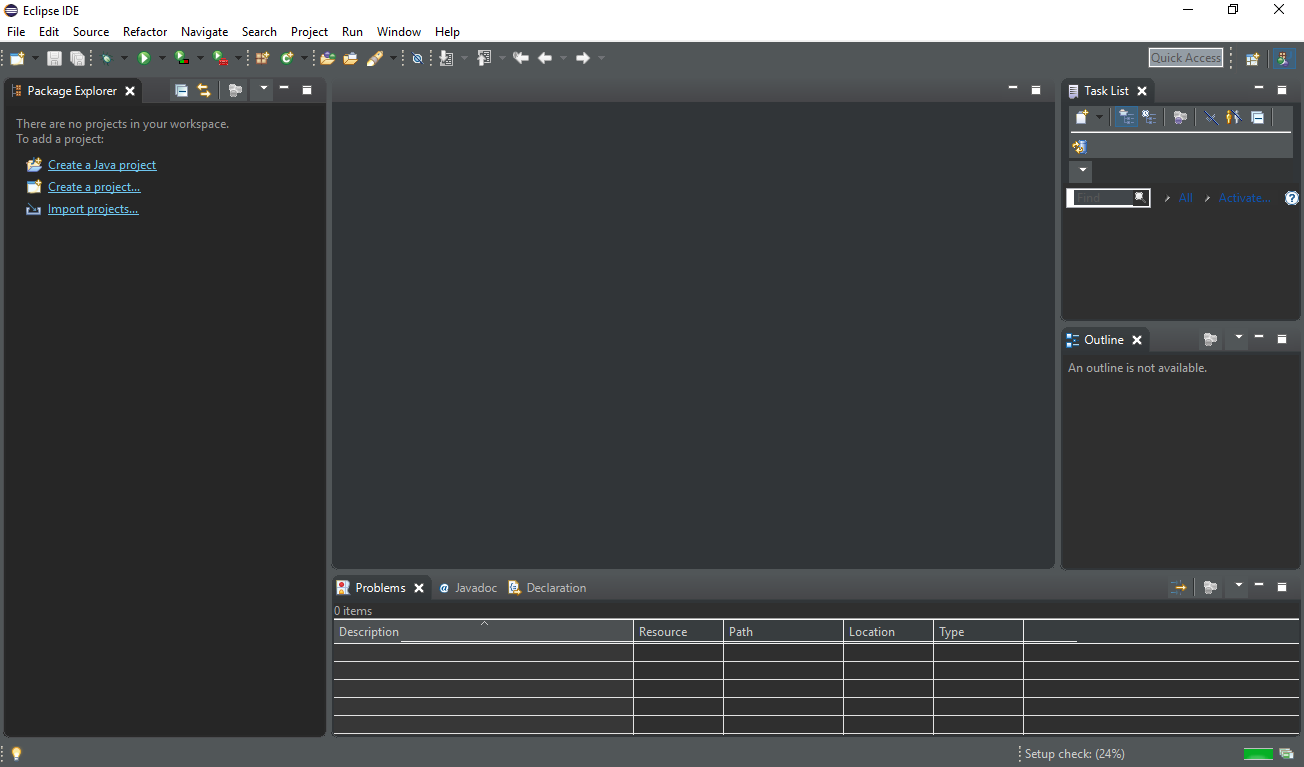
\includegraphics[width=0.8\textwidth]{images/EclipseIDE.png}}
    \caption{Eclipse IDE.}
    \label{fig:eclipseIDE}
\end{figure}

\section{Eclipse PDE}

As mentioned before, Eclipse is mostly known as an IDE. According to Wayne Beaton of Eclipse Foundation \cite{Beaton2013}, however, it was never intended to exclusively be one. It was developed to provide a platform unto which different tools could be integrated. Therefore in fact the core of Eclipse has small functionality by itself and the rest of the tools that are nowadays so broadly used are attached via plugins. That means, Eclipse is designed to be easily extendable. Because of its nature, Eclipse is a perfect tool to be used as a base for general purpose applications. These rich client applications, as well as, plugins for Eclipse core can be developed in Eclipse itself through the use of Plug-in Development Environment (PDE). Once PDE is installed it is enables creation of a new plugin project. The project requires a proper set up at first. Eclipse plugins are based on Open Service Gateway Initiative (OSGi) bundles \cite{Rouse2011}. OSGi is used to manage them in Eclipse application. A plugin must contain a manifest file (\textit{MANIFEST.MF}) with valid OSGi headers for name and version (similarly to Maven). Manifest file is extremely important. It describes the content of a plugin necessary for Eclipse during run-time, such as dependencies, classpath, what is exported \etc Information about the build is held in \textit{build.properties} file. Modular nature of plugins allow them to use other decoupled elements and to be used by other elements as well. This is done by so called extensions and extension points. An extension is \eg a UI element that runs a specific command (which is an extension by itself). CodeSpeech has one UI extension added to the menu - a toggle button that switches the listening on or off. These are managed by another file, namely \textit{plugin.xml}. PDE provides a full featured editor for modifying all three files: \textit{MANIFEST.MF}, \textit{build.properties} and \textit{plugin.xml}.

Once everything is set up, development is focused around a class called the \texttt{Activator}. It is the starting point of any plugin. \texttt{Activator} class extends the \texttt{Plugin} and it is responsible for other classes. The class is initialized whenever any member of the plugin is referenced.

To familiarize the reader with the plugin development using PDE a small example is presented below. The example is explained in detail through the description of the process together with screenshots. The plugin consists of a single toolbar button which displays a message after being clicked. 

\subsection{Necessary software}

As it was mentioned before, the first thing needed is an instance of Eclipse IDE installed in the computer. Eclipse can be downloaded from the official website \footnote{https://www.eclipse.org/eclipseide/}. After that, an enhancement of PDE has to be integrated into the IDE. This can be done via Eclipse Marketplace, accessible from within Eclipse itself, through its menu (Help -> Eclipse Marketplace). In addition to that, yet another software has to be installed, namely Eclipse RCP Target Components. This can be done also through IDE's menu (Help -> Install New Software...). Fig. \ref{fig:eclipseSoftware} show how the corresponding download windows look like. After all of these steps are done, the environment is ready to create a plugin.

\begin{figure}[hbt!]
\centering\small
\begin{tabular}{@{}c@{\hspace{6mm}}c@{}} 
  \fbox{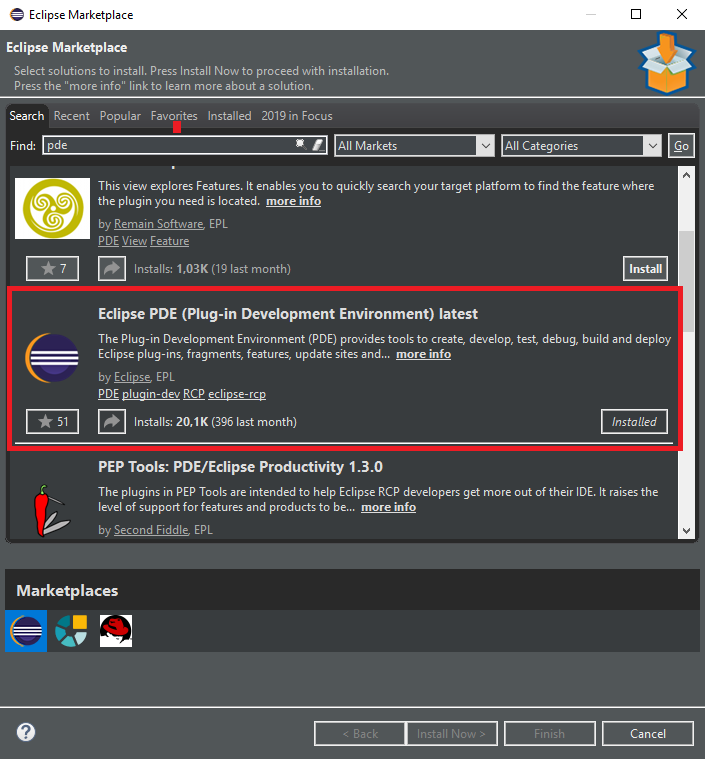
\includegraphics[height=6cm]{images/Tutorial1.png}} &
  \fbox{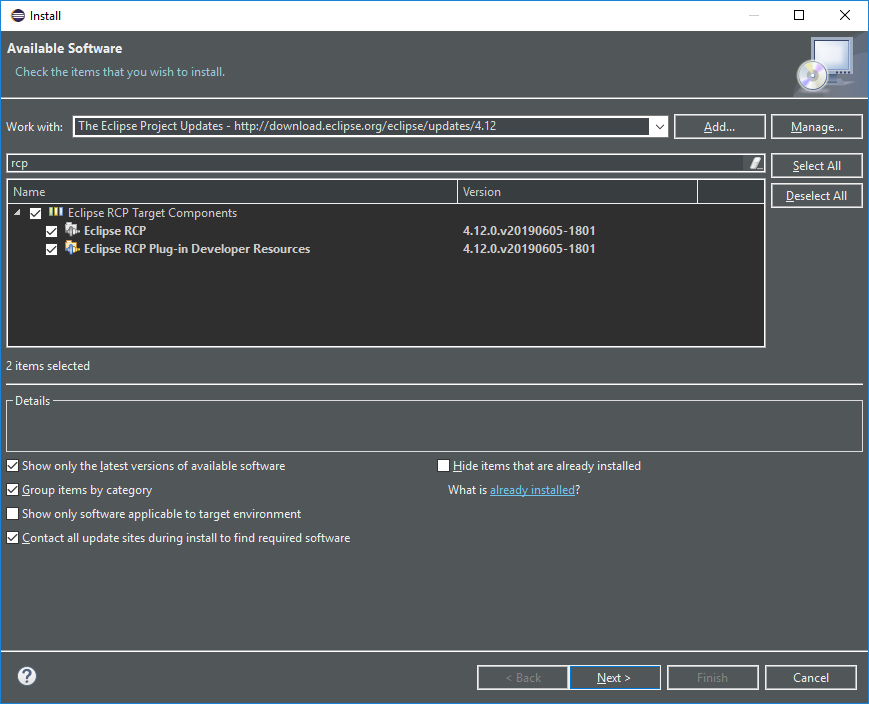
\includegraphics[height=6cm]{images/Tutorial2.png}} 
\\
  (a) & (b)
\end{tabular}
\caption{ Eclipse Marketplace window for PDE donwload (a) and software installation window with Eclipse RCP Target Components Software (b) }
\label{fig:eclipseSoftware}
\end{figure}

\subsection{Project creation}

A plugin can be created in a similar manner as any other type of a project. A creation wizard leads the user through the setup process. The wizard can be opened using menu (File -> New -> Other...). In the pop up window a \textit{Plug-in project} can be selected under the \textit{Plug-in Development} directory. The next consecutive wizard's windows allow for setting up things like plugin's name, id, version as well as setting an \texttt{Activator} and a couple of other options. The last page gives an opportunity to select one of a few plugin templates which comes with some predefined structures. In this example no template is used. Fig. \ref{fig:pluginWizard} shows the sequence of previously mentioned steps.

\begin{figure}[hbt!]
\centering\small
\begin{tabular}{@{}c@{\hspace{3mm}}c@{}} 
  \fbox{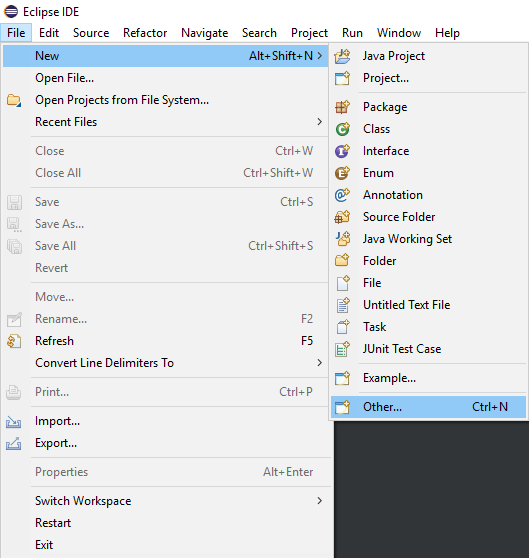
\includegraphics[height=5.5cm]{images/Tutorial3.png}} &
  \fbox{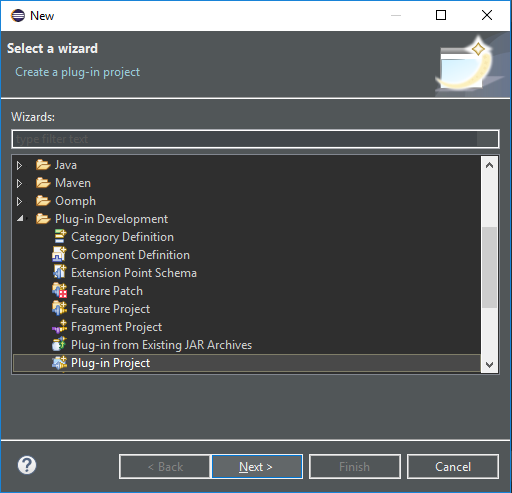
\includegraphics[height=5.5cm]{images/Tutorial4.png}} 
\\
  (a) & (b)
\end{tabular}
  \\[2pt]	
\begin{tabular}{@{}c@{\hspace{3mm}}c@{\hspace{3mm}}c@{}} 
  \fbox{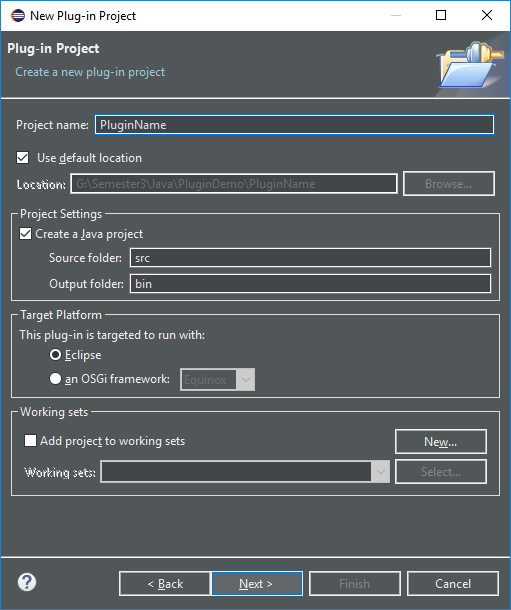
\includegraphics[height=5.5cm]{images/Tutorial5.png}} &
  \fbox{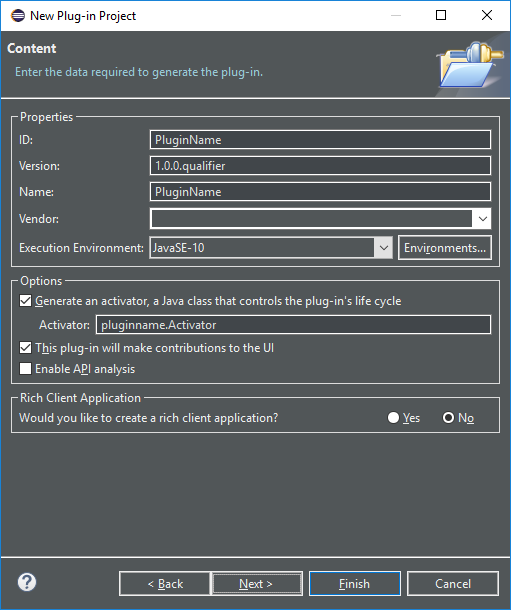
\includegraphics[height=5.5cm]{images/Tutorial6.png}} &
  \fbox{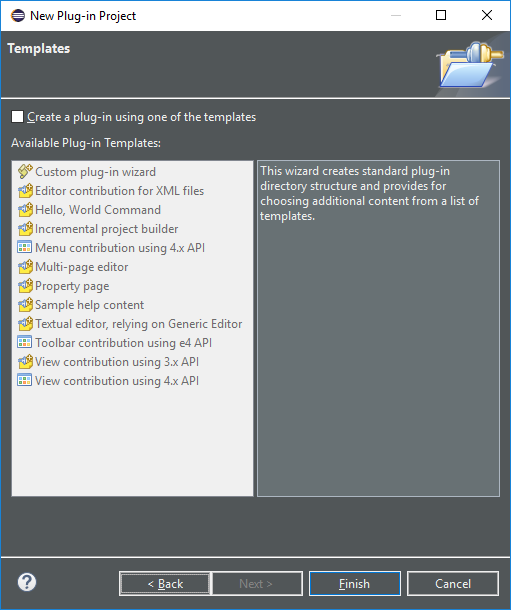
\includegraphics[height=5.5cm]{images/Tutorial7.png}} 
\\
  (c) & (d) & (e)
\end{tabular}
\caption{ Consecutive steps of plugin project creation. Launching creation wizard (a \& b), project options wizard (c), plugin options wizard (d) and template wizard (e). }
\label{fig:pluginWizard}
\end{figure}

Once the project is created it can be seen in \textit{Package Explorer}. It already contains \textit{build.properties} and \textit{MANIFEST.MF} files and \texttt{Activator} class. By clicking on the manifest file a special editor opens up on \textit{Overview} tab. Fig. \ref{fig:pluginProject} presents generated project structure and depicts manifest editor.

\begin{figure}[hbt!]
\centering\small
\begin{tabular}{@{}c@{\hspace{2mm}}c@{}} 
    \fbox{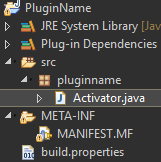
\includegraphics[height=4.5cm]{images/Tutorial8.png}}  &
  \fbox{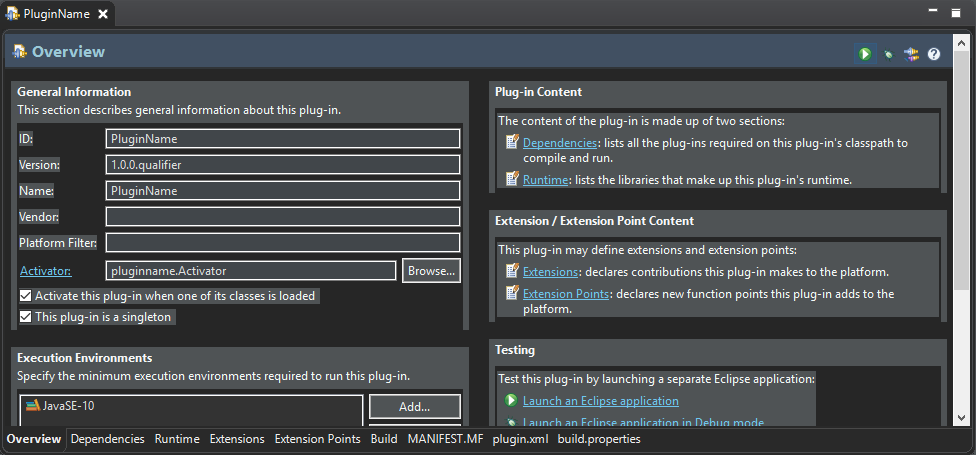
\includegraphics[height=4.5cm]{images/Tutorial9.png}} \\
  (a) & (b)
  \end{tabular}
\caption{ Project structure(a), manifest editor (b). }
\label{fig:pluginProject}
\end{figure}

\subsection{Adding extensions}

Adding a toolbar button requires extending the \textit{org.eclipse.ui.menus} extension point. This can be in the \textit{Extensions} tab, where by clicking the \textit{Add} button another wizard appears. This wizard allows us to browse, search and select necessary extension point. When extension point of interest is found and confirmed with \textit{Finish} button, the new extension point is visible as added into the list. By right-clicking the item a drop down menu is displayed, opening certain options for this item. To add a toolbar, a new menu contribution needs to be created first. Its \textit{locationURI} field must be set to \textit{toolbar:org.eclipse.ui.main.toolbar}. The location specifies where the extension will be placed. The contribution has to be extended by a toolbar with specified id. In order to provide a functionality to it, a command has to be created first. Analogically, at the beginning \textit{org.eclipse.ui.commands} extension point has to be added to the list, then extended by a new command, whose id and name should be specified. Each of the steps is presented in Fig. \ref{fig:menusExtension}.

\begin{figure}[hbt!]
\centering\small
\begin{tabular}{@{}c@{\hspace{3mm}}c@{\hspace{3mm}}c@{}} 
  \fbox{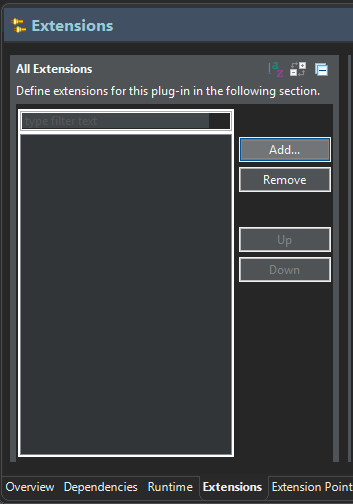
\includegraphics[height=4.8cm]{images/Tutorial10.png}} &
  \fbox{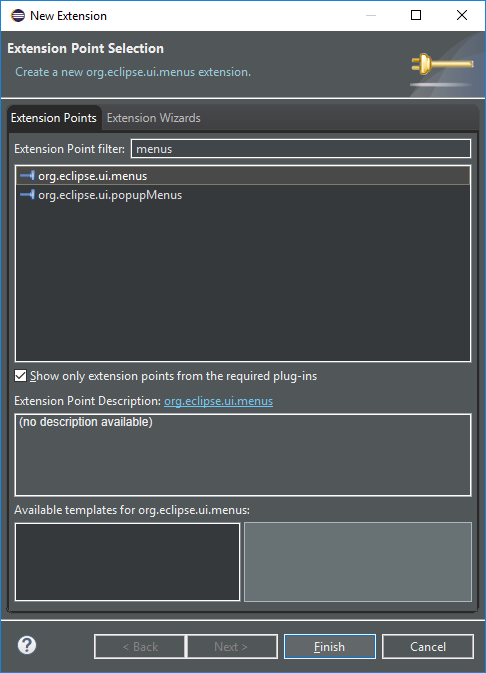
\includegraphics[height=4.8cm]{images/Tutorial11.png}} &
  \fbox{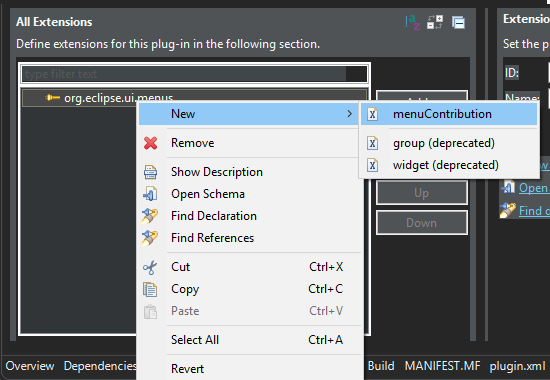
\includegraphics[height=4.8cm]{images/Tutorial12.png}} \\
  (a) & (b) & (c)
  \end{tabular}
  \\[2pt]
\begin{tabular}{@{}c@{\hspace{3mm}}c@{}} 
  \fbox{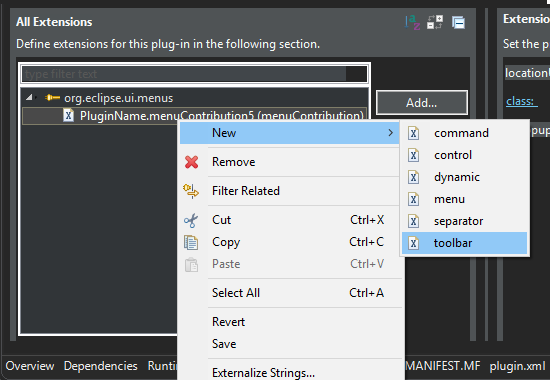
\includegraphics[height=4.8cm]{images/Tutorial13.png}} &
  \fbox{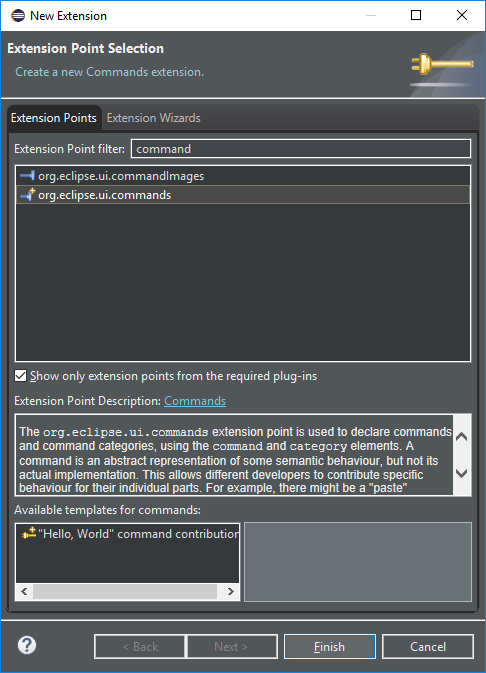
\includegraphics[height=4.8cm]{images/Tutorial14.png}} \\
  (d) & (e) 
  \end{tabular}
\caption{ Extenstion points list in Extenstions tab (a), addition of \textit{org.eclipse.ui.menus} (b), addition of menu contribution and a toolbar (c \& d), addition of \textit{org.eclise.ui.commands} (e).}
\label{fig:menusExtension}
\end{figure}


 When a command is triggered, its handler performs specified action. To assign a handler to the command, its name needs to be put into the \textit{defaultHandler} field (or selected via \textit{Browse} button to the right). In this case a new handler is to be implemented in a form of a new class that extends \texttt{AbstractHandler}. Resulting class presented in Program \ref{list:clickHandler} will only display a dialog with text. Now that the command is created it can be used in a toolbar button. Assigning the command to the toolbar is done in a similar manner as the rest of the extensions. It is important to give correct command's id in a field named \textit{commandId}. These steps are depicted in Fig. \ref{fig:toolbarCommand}.
 An image can be added to the button via \textit{icon} field, this time it is 16x16 pixels \textit{.png} file. If everything was done correctly, the program can be run as ``Eclipse Application''. The plugin's toolbar should be visible in a menu with the chosen image and once clicked, the dialog should appear as shown in Fig. \ref{fig:resultingPlugin}. That concludes the example. More detailed information can be found in the official documentation \cite{eclipse2019}.
 
 \begin{program}[hbt!]
    \caption{Start of interpretation procedure.}
    \label{list:clickHandler}
    \begin{JavaCode}
public class ToolbarClickHandler extends AbstractHandler {
	@Override
	public Object execute(ExecutionEvent event) throws ExecutionException {
		MessageDialog.openInformation(HandlerUtil.getActiveWorkbenchWindow(
                event).getShell(), "Info", "You clicked the button!");
		return null;
	}
}   \end{JavaCode}
\end{program}


\begin{figure}[hbt!]
\centering\small
\begin{tabular}{@{}c@{}} 
  \fbox{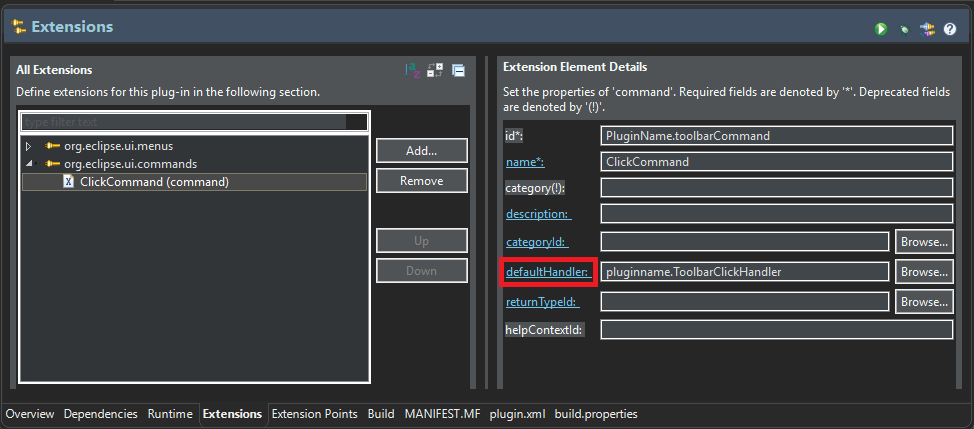
\includegraphics[height=5cm]{images/Tutorial15.png}} \\
  (a) 
  \end{tabular}
  \\[2pt]
\begin{tabular}{@{}c@{\hspace{2mm}}c@{}} 
  \fbox{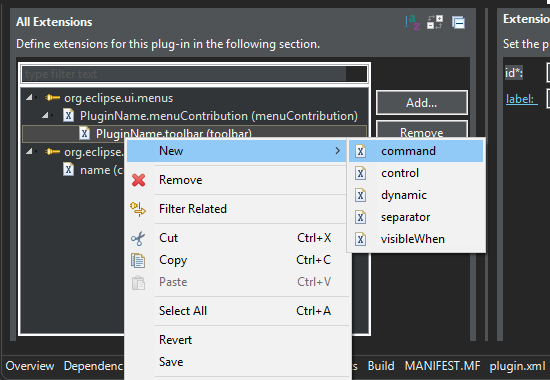
\includegraphics[height=4cm]{images/Tutorial16.png}} &
  \fbox{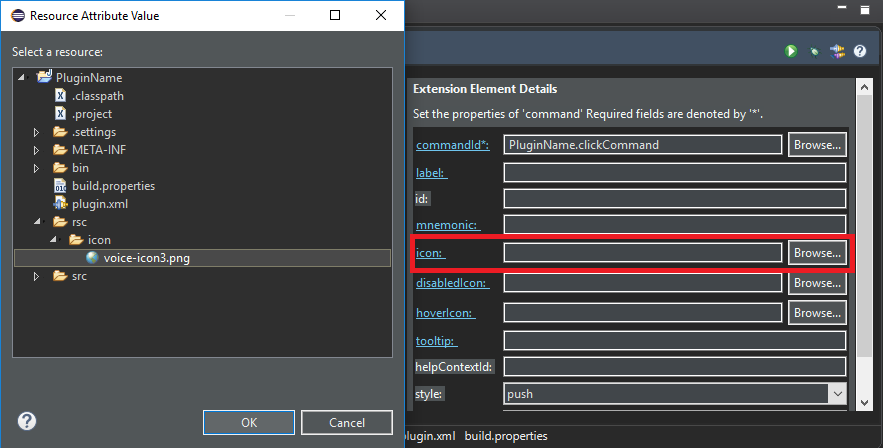
\includegraphics[height=4cm]{images/Tutorial17.png}} \\
  (b) & (c) 
  \end{tabular}
\caption{Field for command's default handler (a). Addition of command to the toolbar (b \& c). }
\label{fig:toolbarCommand}
\end{figure}


\begin{figure}[hbt!]
\centering\small
  \fbox{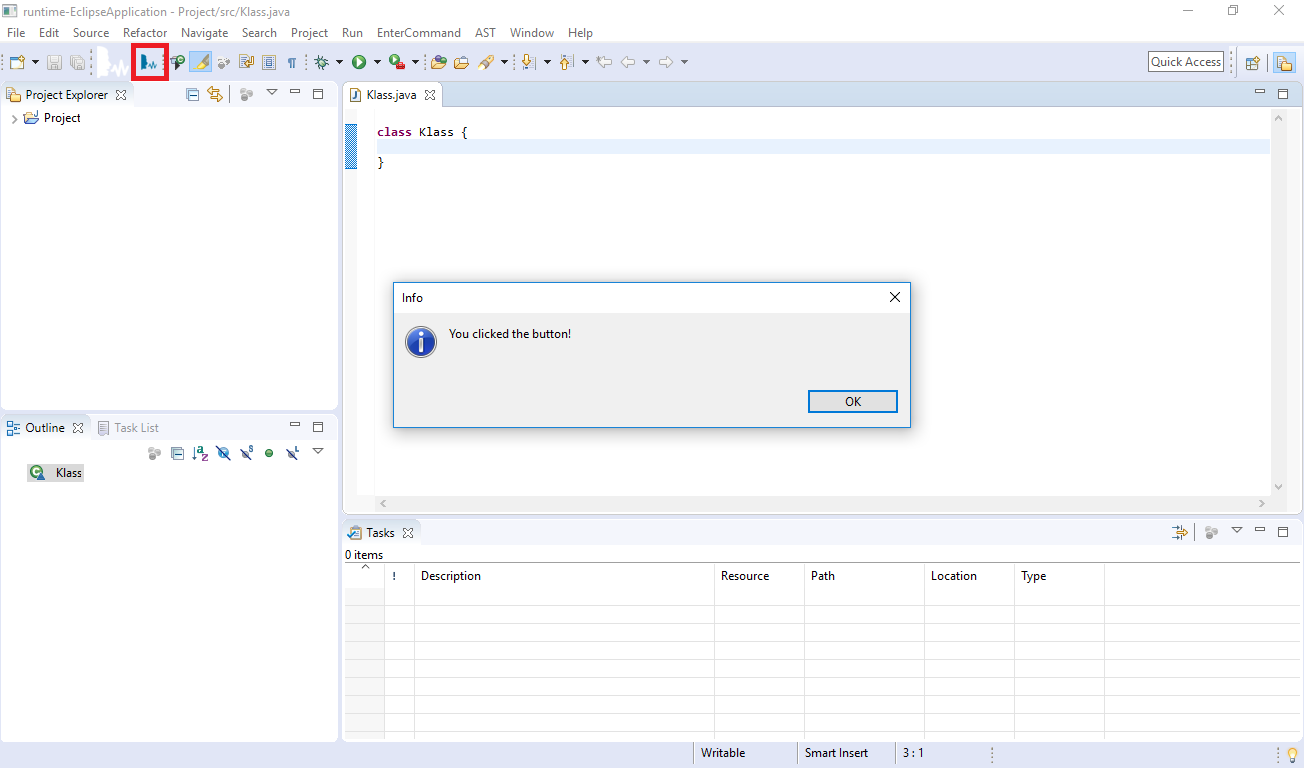
\includegraphics[width=0.9\textwidth]{images/Tutorial18.png}}
\caption{ Resulting plugin. }
\label{fig:resultingPlugin}
\end{figure}

\section{Speech Recognition tools}

Three different speech recognition tools are integrated into the project - two are different implementations of CMUSphinx toolkit, which is open-source and free of charge, and one is using Google Cloud Speech-to-Text API. Subsections below describe each of them in more detail. Before that, however, at the beginning a short introduction into how speech recognition works is given.

\subsection{Explaining speech recognition}

In a nutshell, humans communicate with each other using language. This languages consists of sentences, and these consists of words. Focusing only on the spoken aspect of a language, words are made out of subwords such as syllables, which in turn are made out of units of sound called phonemes. It is a simplification, however, as the sound of the phonemes can vary depending on the speed of speech, context, speaker, accent \etc In English language there are roughly 40 phonemes. It is these elements that the computer tries to match in order to recognize a word. 

At first, a couple of sentences on how voice is being transferred to the computer. Voice is a sound wave created by a vocal apparatus that produces vibrations in the air. A microphone converts the sound into electrical signal. This signal (as the sound itself) is continuous (analog). In order for a computer to understand this signal it has to be converted into a digital one. This is done by analog-to-digital converter (ADC), which performs certain operations such as sampling, filtering, normalization, adjusting to match the speed of a template \etc Once the signal is ready, it is then divided into small portions (frames) of a few hundredths or thousandths of seconds which are a subset of phonemes called senones. These segments are used to match known phonemes.

The rest of the process is belongs to Machine Learning domain. For each frame a number of features are extracted. Each feature is a characteristic aspect of the segment which together with others creates a feature vector - a fingerprint of a kind. These features are used to match a model using complex mathematical functions and probability to determine the most likely outcome. Because of computational limitations and complexity of feature matching, the number of features should be as small as possible, yet the features should be strong enough to enable distinction between the segments. \\
In speech recognition the most commonly used model is called Hidden Markov Model (HMM). During the process of matching each phoneme is assigned a specific probability score based on previously done training and a dictionary. The process does not consider one phoneme at a time, but it also takes into account neighbouring phonemes, therefore it is contextual. It is done on the level of building words, but also the whole phrases.

There are two models that are necessary for speech recognition: acoustic and language model. The former contains acoustic properties for each senone. This model can be context-dependent or context-independent. The latter is used to restrict the search for words by defining which word could follow the one preceding it. In result this significantly quickens the process by focusing on the most probable words. Otherwise, having a vocabulary of 60.000 words and a sequence of three words the program would need to check 216 trillion possibilities. \\ A component that is required to combine these two models provides some sort of a mapping between the phonemes and words. This can either be done by so called phonetic dictionary, which is a list of words with phonemes representing them, or by more efficient complex mathematical function achieved by machine learning algorithm.

\subsection{CMUSphinx}

The initial idea was to base the whole project on available free of charge software elements. An open-source Speech Recognition engine was therefore preferable. After a small research CMUSphinx was selected as it was recommended most often. It was said that it is accurate enough, easy to implement and with very broad documentation. Its documentation is indeed quite well described and is very helpful \cite{CMUSphinx}. It is stated there that CMUSphinx is \textit{leading speech recognition toolkit with various tools used to build speech applications}. On top of that \textit{CMUSphinx contains a number of packages for different tasks and applications}. The toolkit provides different tools, including two recognizer libraries: Pocketsphinx and Sphinx4. Pocketsphinx is a lightweight library written in C, recommended when speed and portability are the main factors or when recognition is to be run on embedded device. Sphinx4 on the other hand is easily adjustable, modifiable recognizer written in Java. It is said that its flexibility makes it possible to quickly build a system. When it comes to selection between the two, it is not accuracy that should be the main criteria but rather the nature of application. In this project Sphinx4 was the first choice mainly for the sole reason, that it is a pure Java library and it is simple to integrate it to Java project, which CodeSpeech is. After further reading, however, the author of this thesis decided to also give Pocketsphinx a try. That is because of the additional recognition method that Pocketsphinx provides which Sphinx4 does not, namely keyphrase recognition. Other two methods that are available for both technologies are continuous speech and grammar based recognition. All three of the previously mentioned methods of recognition will be explained later.


\subsubsection{Sphinx4}

As stated in the documentation, integration of Sphinx4 was relatively easy and quick. The only thing that was needed to use its API were two Java library files, namely sphinx4-data.jar and sphinx4-core.jar. The former consists of acoustic model, dictionary and language model, the latter is API itself. After giving it a try it turned out that recognition of continuous speech did not work well for the author of the thesis. The accuracy, even though not measured, was clearly poor. 

\subsubsection{PocketSphinx}

Integrating PocketSphinx into the project was a completely different story. It lasted for plenty of hours that were spent on solving  continuously coming up issues occurring on different stages. Problems followed the whole process: from correctly building libraries from the source, through usage of Swig to build JNI Java files from C code (although bless the creators of CMUSphinx that this possibility is present and the whole library does not have to be translated to JNI manually) to finally use the generated JNI files as a library in a project. Error messages were often misleading and resulted in additional hours spent on looking for a mistake (which are very easy to make). To be fair, PocketSphinx was never intended to be used in Java projects (that is what Sphinx4 is for), and yet a possibility exists.

When finally all of the necessary libraries were built and loaded, the implementation could be continued. At first an Android project using PocketSphinx available online was used as a template. The accuracy of PocketSphinx was similarly poor to Sphinx4's, nevertheless the results were being returned faster. 

With both technologies giving not satisfying enough results, the author decided to try to adapt models used by CMUSphinx in order to improve the accuracy of the recognition. 

\subsubsection{Model adaptation}

In cases of low accuracy the documentation of CMUSphinx proposes to adapt acoustic model. This can be done relatively easily using Sphinxbase library which \textit{provides common functionality across all CMUSphinx projects}. Sphinxbase is provided together with PocketSphinx package. Adaptation was performed based on corresponding chapter of the documentation. Accordingly, twenty audio transcriptions consisting of the author reading multiple words were recorded, proper text files were created and finally the model was adopted. It did not bring the results that were hoped for, unfortunately, accuracy remained poor. It is possible, that for a significant improvement even more recordings (at least hundred) are necessary, because of time limitation however, this process was skipped. 

Since the adaptation of the acoustic model did not end in significant increase of accuracy of recognition, another means of improvement mentioned in the documentation were performed. These included building a new language model, new dictionary and combination of all three steps. These tasks were quite difficult to do on Windows OS and turned out to be easier on Linux. In the end no success was achieved.

The creators of CMUSphinx explained that the low accuracy might be related to the author's accent. The models were built for American speakers and thus does not work well for people talking differently. Even British people won't be able to achieve high accuracy unless they build a new model their own voices. Building the new model from scratch requires a lot of time, plenty of hours of recordings and is a very complicated process. Due to the limited amount of time it was decided to move on and find another speech recognition tool. 

\subsection{Google Cloud Speech-to-Text}

Google Cloud Speech-to-Text is a service that enables developers to convert audio to text by applying powerful neural network models hosted in a cloud. It recognizes 120 languages and variants, and has an API that is easy to use. On the official website of the service it is possible to try it out before making a decision, and without a doubt this recognition is far better than the one provided by CMUSphinx. API was indeed very simple to integrate to Java project and worked almost out of the bat. This service is not free of charge however. The pricing as it was at the time of writing this thesis is presented in Fig. \ref{fig:cloudSpeechPricing}. As can be seen, there exists a free tier up to 60 minutes of recording that lasts for a year. This is very fortunate, because the initial assumption was to create programming by voice prototype without any money spend. The free tier allows the author to create the prototype and see if the idea of programming by voice in a plugin is possible at all. Once the hypothesis is confirmed, more time can be put into either enhancing current CMUSphinx models, creating a completely new one or applying yet another free-of-charge tool with good enough accuracy.

\begin{figure}[hbt!]
    \centering
    \fbox{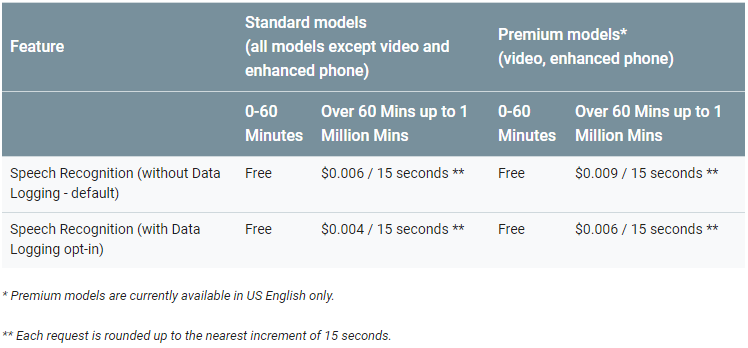
\includegraphics[width=0.85\textwidth]{images/CloudSpeechPricing.png}}
    \caption{Pricing of Google Cloud Speech-to-Text service (taken from official website \cite{CloudSpeech2019}).}
    \label{fig:cloudSpeechPricing}
\end{figure}

Google Speech-to-Text being a cloud service, obviously requires Internet access. The recording of voice is done on the local machine, but once an utterance is finished, it is being sent over to Google server and there neural network models perform recognition. After it is done the result is sent back via callback. That is another difference with previously mentioned technologies, which run entirely on local machine and do not require an Internet connection.

\subsection{Comparison of SR tools}

A summary of certain features belonging to aforementioned tools is presented in the Tab. \ref{tab:comparisonSR}. This table might help in making a decision as to which technology should be used in the development of future Java projects. The difficulty of integration is of course relative, however, the fact that Sphinx4 and Google Cloud Speech-to-Text tools already have existing, ready to use APIs written in Java while PocketSphinx does not, plays a big part here. PocketSphinx library has to be built, then JNI code generated \etc The time needed for for all theses steps might differ depending on the programmers skills and knowledge, nevertheless the number of steps required for integration is significantly higher in comparison to the other two. It is of course understandable as PocketSphinx was never intended to be used for Java projects. \\
In addition, all engines were tested in terms of recognition time and Word Error Rate (WER) metric. The formula for WER is 
 $$   WER = \frac{I + D + S}{N}, $$
where I is the number of inserted words, D is the number of deleted words, S is the number of substituted words and N is the number of words in the original (reference) sentence. In controversial situations like e.g. when one word from the reference text was recognized as n words, one substitution and n - 1 insertions were counted. In a reverse situation, when multiple words were recognized as one, the entry had one substitution and n - 1 deletions. In order for the comparison to be more accurate, test was performed on recordings rather than live speech. The reason for that is to ensure that exactly the same audio is analysed by each software. For this purpose ten sentences were recorded and used by each tool's file analyser. Resulting sentences were written to the file and then WER was manually calculated. 

\begin{table}[hbt!]
    \caption{Comparison of used SR technologies in regard of features important for Java developers.}
    \label{tab:comparisonSR}
    \centering
    \setlength{\textwidth}{5mm} % separator between columns
    \def\arraystretch{1.25} % vertical stretch factor
    \begin{tabular}{|r||c|c|c|}
        \hline
        & \emph{Sphinx4} & \emph{PocketSphinx} & \emph{Google Speech-to-Text} \\
        \hline
        \hline
        Integration difficulty & Easy & Difficult & Easy \\
        \hline
        Price & Free & Free & Free-tier, paid \\
        \hline
        Internet connection & No & No & Required \\
        \hline
        WER [\%] &  88,2 & 94,3 & 17  \\
        \hline
        Average time [s] &  19,76 & 2,12 & 2,17 \\
        \hline
    \end{tabular}
\end{table}

The results of this test show that when it comes to performance Google Cloud Speech-to-Text is clearly the winner. Not only it does the recognition quickly despite the need of sending and receiving data through the Internet, but also has the smallest WER score of 17\%. PocketSphinx recognizes in a similar speed (in this experiment slightly faster), but its WER is very high (around 95\%). Sphinx4 did a bit better than PocketSphinx in terms of recognition, but was incredibly slow (almost 10 times slower than the other two). Taking all that into consideration, Google Cloud Speech-to-Text was used as a main speech recognition engine, although all three were integrated into the system. Perhaps in the future CMUSphinx models will be trained to increase the performance.

\section{ANTLR}

The end goal of the finished programming by voice product is to perform operations using natural sentences. At the end of the previous chapter an issue related to the way code is read by different people is discussed. The same problem might appear when it comes to steering the program by voice through the use of different commands. Taking that into consideration, it was decided that for the control over the program by voice commands an interpretation of specified grammar will be used. Although grammars are usually quite strict when it comes to token recognition because each of the required elements must occur in a right position, they also allow a certain amount of flexibility by enabling representation of tokens by different keywords/phrases. Once decided upon this approach, a proper tool had to be selected for parsing and managing grammars and finally the choice was ANTLR (ANother Tool for Language Recognition). ANTLR as described on the official website 
\begin{quote}
    \begin{english}
   is a powerful parser generator for reading, processing, executing, or translating structured text or binary files. It's widely used to build languages, tools, and frameworks. From a grammar, ANTLR generates a parser that can build and walk parse trees \cite{ANTLR2019}.
    \end{english}
 \end{quote}
ANTLR turned out to be exactly what was needed, giving a lot of options in the way the sentence is parsed. This flexibility is a great advantage of ANTLR. Below more information about working with ANTLR are given.

\subsection{Typical workflow}

At first ANTLR tools have to be installed and then grammar file with \textit{.g4} extension created. Then, running ANTLR tools against the grammar generates code that enables handling each specific token or keyword at any time. Whenever the change in grammar is made, new files have to be generated and applied to the project. The most important from the point of view of developer are listeners or visitors files (depending on the option). They provide methods that are triggered whenever a token is entered or exited. Many custom listeners or visitors can be implemented, each allowing for alternative interpretation of the same token depending on a current state of the program. The whole process was divided into three parts: installation of ANTLR tools, writing a grammar and generation of the files.

\subsubsection{ANTLR tools}

ANTLR consists of two parts: the tool used to generate lexer and parser, and the runtime needed to run them by the end software. The tool is the Java program and it requires at least Java 1.7 installed on a working machine. To install the program it needs to be downloaded from the official website from a download section and then added to the classpath of the system. When done, \texttt{antlr4 <options> <grammar-file-g4>} command can be used in order to generate files needed by the end software. Options allow generation thereof to a specific language other than Java (which is set as default) \eg Python or JavaScript, or to choose between generation of listeners (default) or visitors. \\
This is one way of using ANTLR. During this project yet another approach was used. Generation of needed files based on the grammar was done through another external ANTLR project. It is a simple Java project which uses ANTLR libraries via Maven. The grammar is placed in project's \textit{src/main/antlr4} folder. Generation is then done using \texttt{mvn package} command. 

The end Java program that will use ANTLR can be set up either by Gradle, Maven or manually. Because of the conflict that occurs between Eclipse plugin project and other manifest-based ones, for now the CodeSpeech is set up manually. Addition of external libraries such as antlr4-runtime.jar to Eclipse plugin project can be done via \textit{Runtime} tab of the manifest editor in the \textit{Classpath} area as shown in Fig. \ref{fig:jarAddition}.

\begin{figure}[hbt!]
    \centering
    \fbox{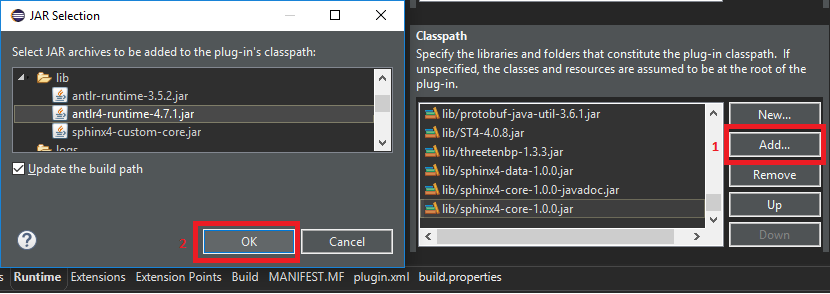
\includegraphics[width=\textwidth]{images/ANTLR1.png}}
    \caption{Addition of external library. }
    \label{fig:jarAddition}
\end{figure}

\subsubsection{Grammar}

Grammar consists of lexer and parser rules. Lexer, also known as tokenizer analyzes text and assigns a proper token to parts of it. Parser takes these tokens and organizes them into abstract syntax tree. Both parser and lexer perform their tasks using so called rules. In ANTLR lexer and parser rules are distinguished by the first character of the rule's name: parser rules start with lower case and lexer rules with upper case. For better readability it is common to write the name of the lexer rules completely in upper case. Lexer rules are usually put at the bottom of the grammar, however, from the ANTLR's point of view it does not matter, it is just a standard of organization. It is possible to divide parser and lexer rules to two separate files. In Program \ref{list:grammar} both types of rules are in one file, with lexer rules being at the bottom. 

\begin{program} [hbt!]
    \caption{Example of grammar file's content. This grammar allows creation of simple mathematical equations. }
    \label{list:grammar}
    \begin{JavaCode}
grammar BasicMath;		

/*
 * Parser Rules
 */
program:	(equation NEWLINE)* ;
equation:	equation ('*'|'/') equation
    |	equation ('+'|'-') equation
    |	INT
    |	'(' equation ')'
    ;

/*
 * Lexer Rules
 */
fragment DIGIT : [0-9] ;
INT     : DIGIT+ ; 
NEWLINE : [\r\n]+ ;
WHITESPACE : (' ' | '\t') ;    \end{JavaCode}
\end{program}

As it can be seen, the content of a rule is placed between a colon and a semi-colon defined after the name. A \texttt{fragment} rule allows to create reusable blocks for lexer rules. Parser rule can consist of parser and lexer rules. It can also be seen that ANTLR allows recursion, so referencing itself in the rule. A few symbols that exist in this example are: ``|'' for an alternative, ``+'' for one or more occurrence, ``*'' for zero or more, parentheses for definition of a subrule. Characters, whole words or phrases that are to be recognized are defined in single quotes. More examples, symbols and other interesting information can be found in the official documentation \cite{ANTLRDOC2019}.

\subsubsection{Generation}

Once the grammar is finished a time has come for generation. Without regard for the method of performing that procedure (two were mentioned before), the generated files have to be moved to the project source folder in order to be used. Every time the grammar is modified, the process has to be repeated to apply the changes. This occurs quite often during the development and might be bothersome, however, a simple shell script can help in automation of the whole procedure, which in the end can save a lot of time. The script at first initializes generation by running \texttt{mvn package} in the home folder of ANTLR project. Then it adds proper package name via combination of \texttt{echo}, \texttt{cat} and \texttt{mv} commands and later moves them, to the target directory via \texttt{mv}. This solution speeds up the process, leaving refreshing the project as the only thing to do. 

The generated files are named according to the grammar's file name. If the grammar is named \textit{BasicMath}, then the resulting files will be \textit{BasicMathLexer.java}, \textit{BasicMathParser.java}, \textit{BasicMathListener.java} and \textit{BasicMathBaseListener.java}. File extension of course depends on the selected target programming language. In case of choosing visitors to be created those would replace listener files. In addition, \textit{.interp} and \textit{.tokens} files appear, but those are not needed by the runtime. Program \ref{list:listener} presents an interface contained in \textit{BasicMathListener.java} file. Its implementation in form of abstract class is consisted in \textit{BasicMathBaseListener.java}.

\begin{program} [hbt!]
    \caption{A generated listener. }
    \label{list:listener}
    \begin{JavaCode}
// Generated from BasicMath.g4 by ANTLR 4.7.1
import org.antlr.v4.runtime.tree.ParseTreeListener;

/**
 * This interface defines a complete listener for a parse tree produced by
 * {@link BasicMathParser}.
 */
public interface BasicMathListener extends ParseTreeListener {
	/**
	 * Enter a parse tree produced by {@link BasicMathParser#program}.
	 * @param ctx the parse tree
	 */
	void enterProgram(BasicMathParser.ProgramContext ctx);
	/**
	 * Exit a parse tree produced by {@link BasicMathParser#program}.
	 * @param ctx the parse tree
	 */
	void exitProgram(BasicMathParser.ProgramContext ctx);
	/**
	 * Enter a parse tree produced by {@link BasicMathParser#equation}.
	 * @param ctx the parse tree
	 */
	void enterEquation(BasicMathParser.EquationContext ctx);
	/**
	 * Exit a parse tree produced by {@link BasicMathParser#equation}.
	 * @param ctx the parse tree
	 */
	void exitEquation(BasicMathParser.EquationContext ctx);
}    \end{JavaCode}
\end{program}

As it can be seen, for each parser rule there exist two methods: for entering and exiting specified parser rule. This allows the end program for performing specific actions depending on the implementation. Because many custom listeners can be created and changed back and forth during runtime, a different operation can be performed on the same keyword depending on the context. This elasticity of ANTLR, as well as ease of use, well written and broad documentation and active support were the main factors that decided upon selecting ANTLR as an interpretation tool. 

\subsection{ANLTR plugin}

To make the work with ANTLR easier, it can also be integrated into many IDEs. There exists a plugin for Eclipse called \textit{AntlrDT Tools Suite for Eclipse}, which provides following features:

\begin{itemize}
   \item Advanced Syntax Highlighting
   \item Automatic Code Generation (on save)
   \item Manual Code Generation (through External Tools menu)
   \item Code Formatter (Ctrl+Shift+F)
   \item Syntax Diagrams
   \item Advanced Rule Navigation between files (F3 or Ctrl+Click over a rule)
   \item Quick fixes
\end{itemize}

Syntax diagram is a very helpful feature which helps to visualise how the grammar is constructed. An example can be seen in Fig. \ref{fig:grammarSyntaxDiagram}.

\begin{figure}[hbt!]
    \centering
    \fbox{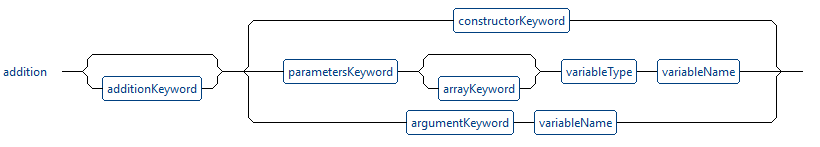
\includegraphics[width=\textwidth]{images/GrammarSyntaxDiagram.PNG}}
    \caption{An example of syntax diagram.}
    \label{fig:grammarSyntaxDiagram}
\end{figure}
